\documentclass[a4paper,11pt]{article}
\usepackage[utf8x]{inputenc}
\usepackage[T1]{fontenc}
\usepackage[french]{babel} 
\usepackage{color}
\usepackage{anysize}
\usepackage{lmodern} % Pour changer le pack de police
\usepackage{makeidx}
\date{} % Pour mettre la date du jour, tapez \today 
\usepackage{verbatim}
\usepackage{graphicx}
\usepackage{epstopdf}
\usepackage{titlesec}
\usepackage[dvipsnames]{xcolor}
\usepackage{wrapfig}
\usepackage[linesnumbered]{algorithm2e} %pr le pseudo code
 \usepackage{amsmath}
 \usepackage{amsfonts}
\usepackage{array}
% les pacakage ci dessous permettent d'aller directement au liens
\usepackage{url} % aller sur le site web


\usepackage[colorlinks=true,linkcolor=PineGreen, urlcolor=PineGreen, citecolor=PineGreen]{hyperref} %aller dans un lien interne

%************ section in green *****************
\titleformat{\section}
{\color{PineGreen}\normalfont\Large\bfseries}
{\color{PineGreen}\thesection}{1em}{}
%************************************************
\begin{document}

\fontfamily{phv}\selectfont

\begin{titlepage}


\includegraphics {./img/depinfo.png} \hspace*{\stretch{1}}
\includegraphics [width=6cm, height=4cm]{./img/UCP_logo_noir}

\vspace*{\stretch{1.5}}

\hrule
\begin{center}\huge\bfseries
\color{PineGreen}{}
TP TSI+ : Filtrage de signaux audio
\end{center}
\hrule
\vspace*{\stretch{0.2}}
\begin{flushleft}
Alexandre FAUCHER \\ Gada REZGUI
\end{flushleft}
\vspace*{\stretch{1.5}}
\begin{center} 
Encadrant :
Ghilès MOSTAFAOUI

\end{center}
\end{titlepage}
\tableofcontents
\newpage

\textbf{Observer le module de la transformée de Fourier. Quelle est la bande de fréquence utile pour le signal ?}
\begin{figure}[h]
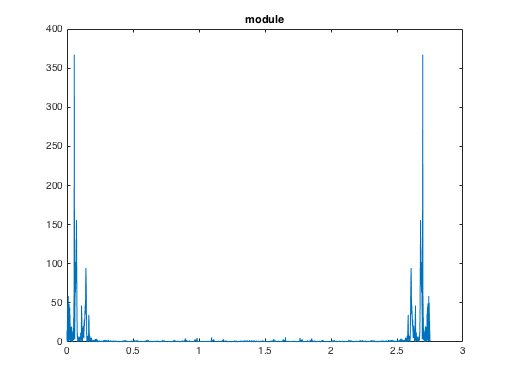
\includegraphics [width=.9\linewidth]{./img/module}
\caption{Module du signal issu de coucou.wav}
\end{figure}

La bande de fréquence utile pour le signal est [0 2.8]
\section{Filtre passe bas à réponse impulsionnelle finie}


\subsection{ Partie théorique}
Soit le filtre passe bas à réponse impulsionnelle finie :
y(k) = x(k)+x(k-1)+...+x(k-D)\\

Écrire ce filtre sous forme récursive.

\begin{math}
y(k) = x(k)+x(k-1)+...+x(k-D)\\
y(k-1) = x(k-1)+x(k-2)+...+x(k-(D+1))\\
y(k) = x(k)+y(k-1)-x(k-(D+1))\\
y(k) - y(k-1)= x(k)-x(k-(D+1))\\
Y(z) - z^{-1}Y(z)  = X(z)-z^{-(D+1)}X(z)\\
Y(z) (1- z^{-1}) = X(z)(1-z^{-(D+1)})\\
Y(z)=\frac{1-z^{-(D+1)}}{1- z^{-1}}X(z) \\
\end{math}

Fonction de transfert :\\
$H(z)=\frac{1-z^{-(D+1)}}{1- z^{-1}}$\\

Module : \\
$H(f)=\frac{1-e^{-2\pi jfTe(D+1)}}{1- e^{-2\pi jfTe}}\\
|H(f)|=\frac{|1-cos(2\pi jfTe(D+1))+j sin(2\pi jfTe(D+1))|}{|1-cos(2\pi jfTe)+j sin(2\pi jfTe)|}\\
|H(f)|=\frac{(1-cos(2\pi jfTe(D+1)))^{2}+ sin^{2}(2\pi jfTe(D+1))}{(1-cos(2\pi jfTe))^{2}+ sin^{2}(2\pi jfTe)}\\
|H(f)|=\frac{2-2cos(2\pi jfTe(D+1))}{2-2cos(2\pi jfTe)}\\
$

\section{Filtre en peigne}

\section{Filtre passe Tout}

\section{Réverbération}

\end{document}
